To quantitatively validate the predicted edge maps against the expert-annotated boundaries, the data-analysis phase of Zotin et al. \cite{zotin2018edge} is formalized using the confusion-matrix quantities \gls{tp}, \gls{tn}, \gls{fp}, \gls{fn} (denoted $\mathrm{TP}$, $\mathrm{TN}$, $\mathrm{FP}$, $\mathrm{FN}$ from here on), and the reference edge count $\mathrm{RECnt}=\mathrm{TP}+\mathrm{FN}$. The percentage of correctly detected pixels ($\mathrm{Pcd}$), the percentage of non-detected pixels ($\mathrm{Pnd}$), the percentage of false alarms ($\mathrm{Pfa}$), Sensitivity, Accuracy, and the \gls{fom} \cite{pratt1979quantitative} are computed as
\begin{equation}
\mathrm{Pcd} = \mathrm{Sensitivity} = \frac{\mathrm{TP}}{\mathrm{RECnt}}\\[0.5em] \quad
\end{equation}
\begin{equation}
	\mathrm{Pnd} = \frac{\mathrm{FN}}{\mathrm{RECnt}}\\[0.5em] \quad
\end{equation}
\begin{equation}
	\mathrm{Pfa} = \frac{\mathrm{FP}}{\mathrm{RECnt}}\\[0.5em] \quad
\end{equation}
\begin{equation}
	\mathrm{Accuracy} = \frac{\mathrm{TP}+\mathrm{TN}}{\mathrm{TP}+\mathrm{TN}+\mathrm{FP}+\mathrm{FN}}
	\\[0.5em] \quad
\end{equation}
\begin{equation}
	\mathrm{FOM} = \frac{1}{\max(\mathrm{RECnt},\mathrm{AECnt})}\sum_{i=1}^{\mathrm{AECnt}} \frac{1}{1+\alpha d_i^2}
\end{equation}

where $\mathrm{AECnt}$ is the number of detected edge pixels, $d_i$ is the distance of the $i$-th detected pixel to its nearest reference edge pixel, and $\alpha=1/9$ is Pratt's empirically calibrated constant \cite{pratt1979quantitative}. Since $\mathrm{Pcd}$ and Sensitivity share the same definition, they are numerically identical and are reported interchangeably. The baseline pipeline is a strict reproduction of \cite{zotin2018edge}, but it is validated on a scale two orders of magnitude larger than the original study: 484 multiparametric volumes (T1, T1Gd, T2, \gls{flair}, with expert-annotated masks) from the Brain Tumor task of the \gls{msd} \cite{antonelli2022medical}, against the 30 hand-picked images used by Zotin et al. For each patient, the T2 channel is extracted and a single fixed axial slice at the volumetric midpoint is processed, mirroring the 2-D, per-image nature of the original study. Two additions, left unspecified by \cite{zotin2018edge}, were required to make the pipeline operate on this dataset. In the baseline (and also for the optimized pipeline next in \ref{sec:optimized}), predicted edges are highlighted in red, expert ground truth in green, and their combined overlay -if they match- in yellow, for the best, median, and worst \gls{fom} cases over the 484 BRATS patients. First, unlike the pre-cropped images used in the original work, \gls{msd} volumes contain a large all-zero background outside the skull; a robust brain mask, obtained via Otsu thresholding followed by hole-filling and largest-component extraction, restricts both the \gls{bcet} statistics and the \gls{fcm} clustering to intracranial tissue. Second, since \cite{zotin2018edge} neither specifies the number of clusters $c$ nor a rule for selecting the tumor cluster once \gls{fcm} has converged, $c$ is fixed at 4, consistent with Gonzalez and Woods' treatment of clustering-based segmentation, where the number of clusters is specified directly rather than estimated automatically. The tumor candidate is then selected among the brightest clusters by scoring the solidity times the area of their largest connected component, excluding any cluster occupying more than 40\% of the brain mask, since the normal brain-tissue cluster is itself large and solid and would otherwise be mistaken for the lesion. Figure \ref{fig:baseline_pipeline} shows every stage of this pipeline applied to a single patient. Panel (\ref{fig:baseline_input}) shows the input T2 slice alongside the radiologist's annotation; panel (\ref{fig:baseline_preprocessing}) shows the result of median filtering, Otsu brain masking, and BCET enhancement; panel (\ref{fig:baseline_segmentation}) shows the four-class FCM segmentation and the isolated tumor candidate; panel (\ref{fig:baseline_edge_extraction}) shows the morphological boundary extracted from this candidate, overlaid on the original slice; and panel (\ref{fig:baseline_validation}) compares this predicted boundary against the expert ground truth.
\begin{figure}[htbp]
    \centering
    \captionsetup[subfigure]{justification=centering} 
    \begin{subfigure}[b]{\columnwidth}
        \centering
        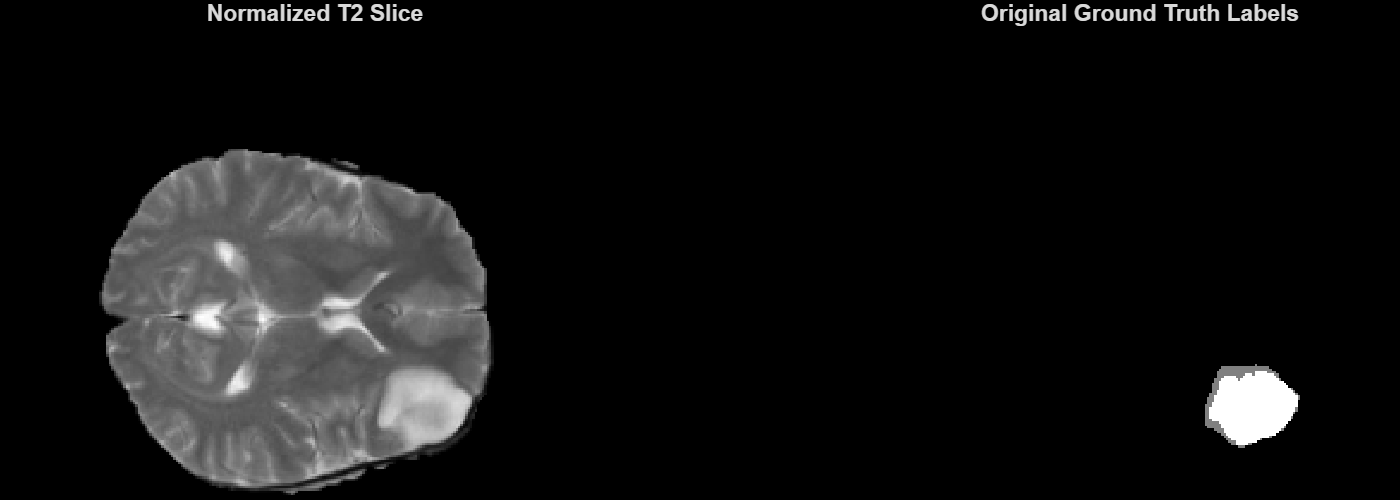
\includegraphics[width=0.9\linewidth]{images/baseline/best_case/01_data_understanding.png}
        \caption[Baseline Input]{Baseline Input: normalized T2 slice and expert-annotated ground truth}
        \label{fig:baseline_input}
    \end{subfigure}
    \vspace{0.1cm} % Spazio ridotto per evitare l'overflow verticale
    \begin{subfigure}[b]{\columnwidth}
        \centering
        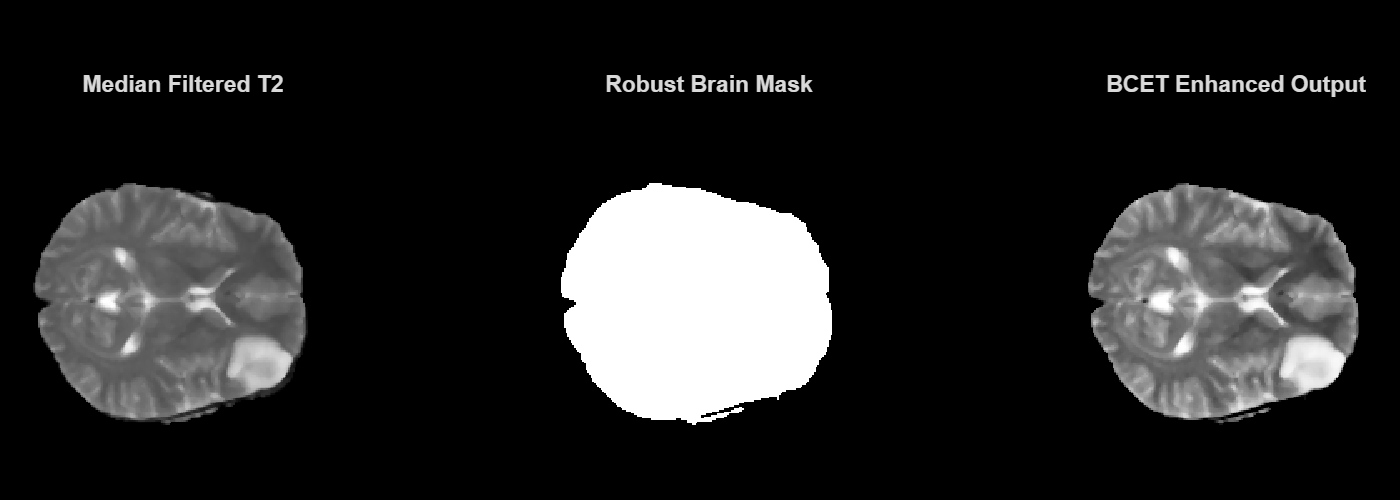
\includegraphics[width=0.9\linewidth]{images/baseline/best_case/02_enhancement.png}
        \caption[Pre-processing]{Pre-processing: median filter, Otsu brain mask, BCET enhancement}
        \label{fig:baseline_preprocessing}
    \end{subfigure}
    \vspace{0.1cm}
    \begin{subfigure}[b]{\columnwidth}
        \centering
        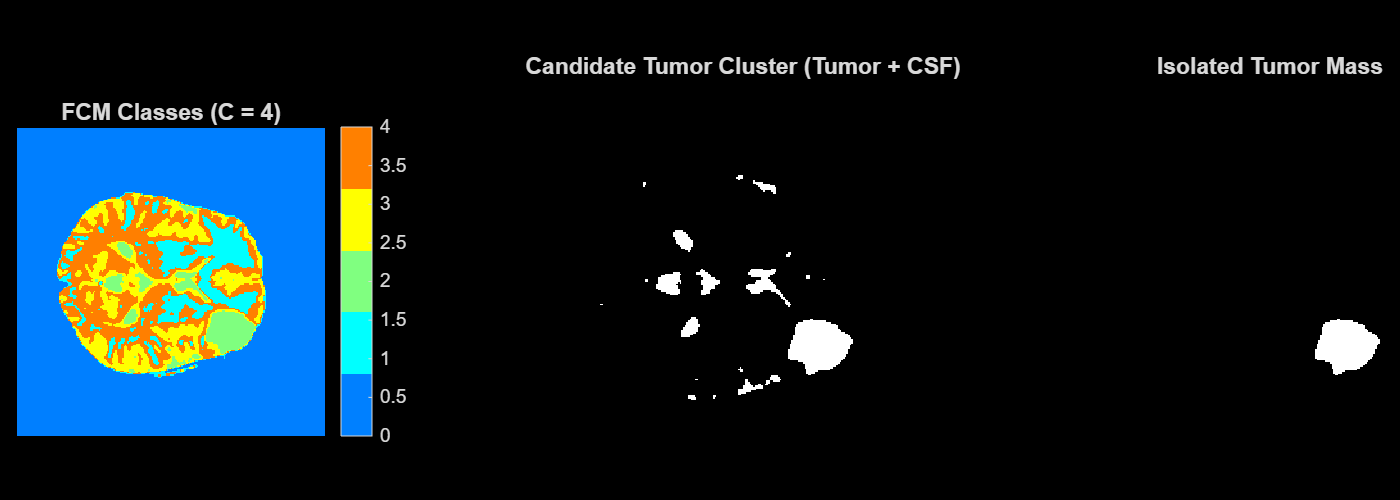
\includegraphics[width=0.9\linewidth]{images/baseline/best_case/03_segmentation.png}
        \caption{Four-class FCM segmentation and tumor-candidate isolation}
        \label{fig:baseline_segmentation}
    \end{subfigure}
    \vspace{0.1cm}
    \begin{subfigure}[b]{\columnwidth}
        \centering
        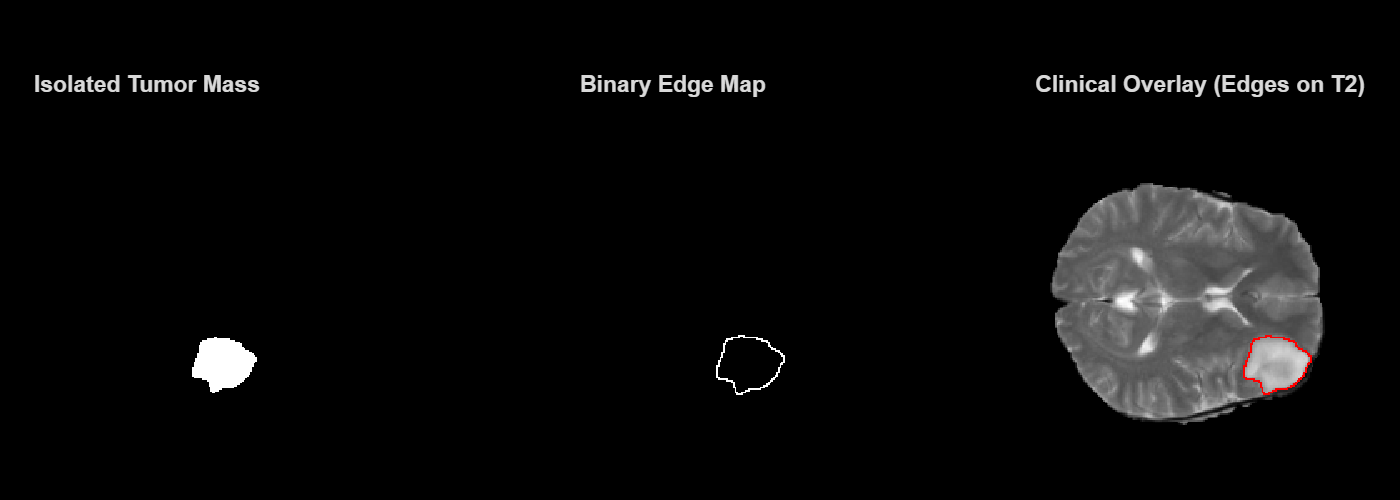
\includegraphics[width=0.9\linewidth]{images/baseline/best_case/04_edge_detection.png}
        \caption{Morphological edge extraction and clinical overlay}
        \label{fig:baseline_edge_extraction}
    \end{subfigure}
    \vspace{0.1cm}
    \begin{subfigure}[b]{\columnwidth}
        \centering
        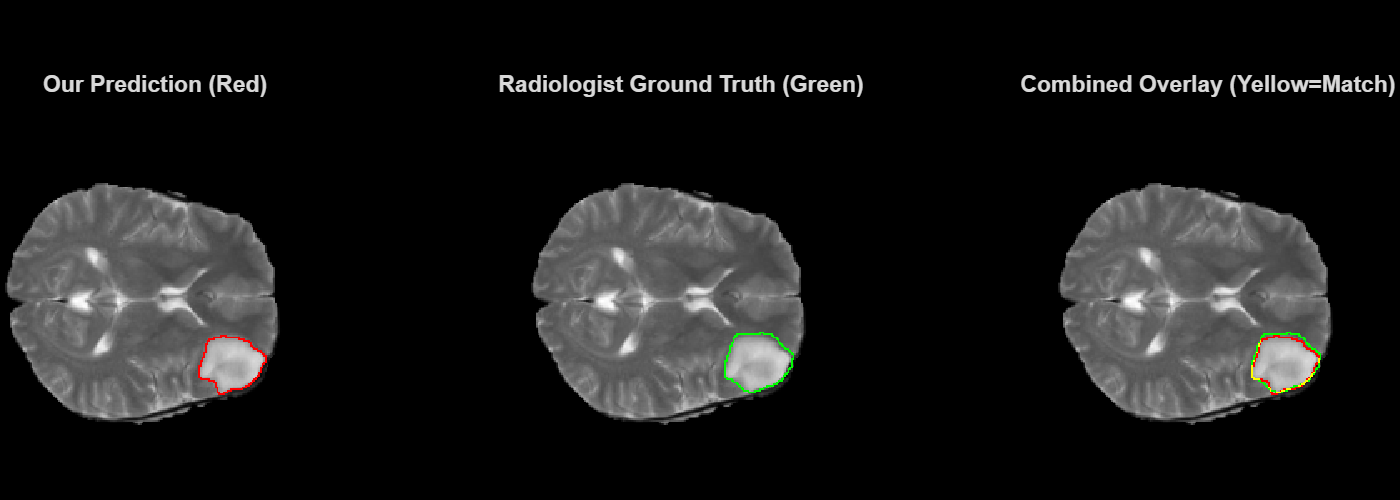
\includegraphics[width=0.9\linewidth]{images/baseline/best_case/05_final_validation.png}
        \caption{Validation: predicted boundary vs. expert ground truth}
        \label{fig:baseline_validation}
    \end{subfigure}
    \caption{End-to-end baseline on patient BRATS\_025 (best \gls{fom} case)}
    \label{fig:baseline_pipeline}
\end{figure}
 Because glioblastomas often outgrow their own blood supply, their core frequently becomes necrotic and hypointense rather than hyperintense, which can split the bright tumor candidate into a ring with a dark hole rather than a solid disc; the largest connected component is therefore hole-filled before isolation, so that the subsequent edge extraction traces only the outer boundary of the whole tumor, matching the convention used by the expert annotation. Finally, because the isolated tumor mask is already binary, a classical Canny detector would degenerate to simple perimeter tracing; a morphological edge detector (dilation of the mask minus the mask itself) is used instead, and applied identically to the reference mask, so that predicted and ground-truth boundaries are extracted with the same operator.\\
 Figure \ref{fig:validation_results} shows the comparison between three different cases: 
\begin{itemize}
    \item \textbf{best case}:the patient with the absolute highest FOM.
    \item \textbf{median case}:the patient whose FOM is as close as possible to the statistical median of all 484 values.
    \item \textbf{worst case}: the patient with the lowest FOM.
\end{itemize}
the predicted edges are in red, the expert ground truth is in green, and their combined overlay is yellow if both spatially match. The comparison is being made for the best, the median, and the worst \gls{fom} cases over the 484 BRATS patients.
\begin{figure}[htbp]
    \centering
    \captionsetup[subfigure]{justification=centering} 
    \begin{subfigure}[b]{\columnwidth}
        \centering
        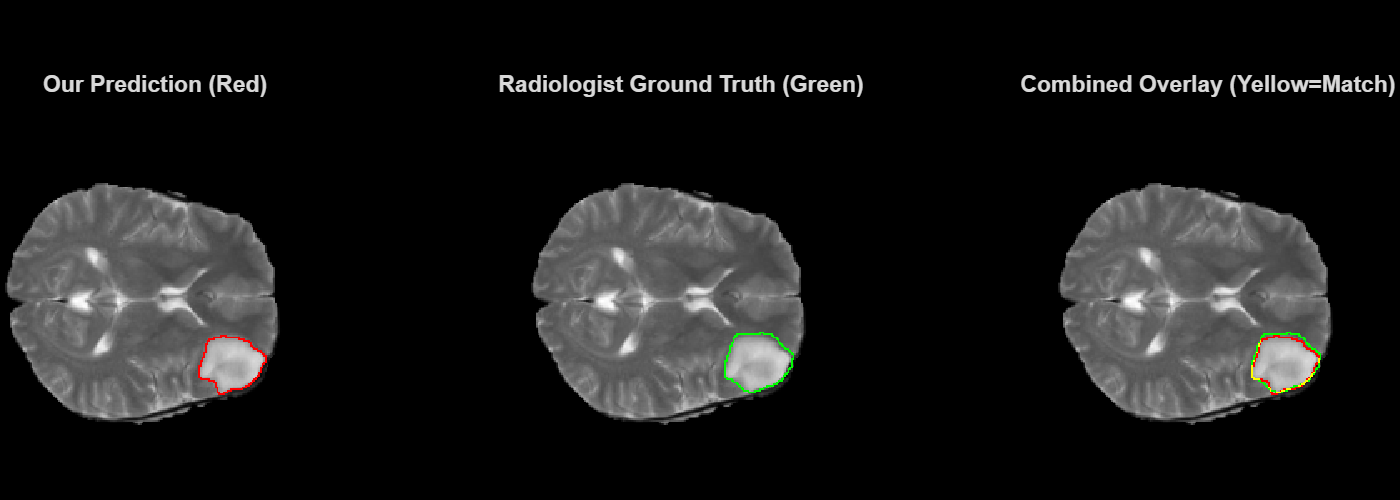
\includegraphics[width=0.9\linewidth]{images/baseline/best_case/05_final_validation.png}
        \caption{Best case: BRATS\_025 ($\mathrm{FOM}=0.847$)}
        \label{fig:baseline_best_cases}
    \end{subfigure}
    \vspace{0.1cm} 
    \begin{subfigure}[b]{\columnwidth}
        \centering
        
\includegraphics[width=0.9\linewidth]{images/baseline/median/05_final_validation.png}
        \caption{Median case: BRATS\_004 ($\mathrm{FOM}=0.136$)}
        \label{fig:baseline_median_cases}
    \end{subfigure}
    \vspace{0.1cm}
    \begin{subfigure}[b]{\columnwidth}
        \centering
        
\includegraphics[width=0.9\linewidth]{images/baseline/worst_case/05_final_validation.png}
        \caption{Worst case: BRATS\_012 ($\mathrm{FOM}=0.000$)}
        \label{fig:baseline_worst_cases}
    \end{subfigure}
    \caption{Baseline comparison between best case \ref{fig:baseline_best_cases}, median case \ref{fig:baseline_median_cases} and worst case \ref{fig:baseline_worst_cases}}
    \label{fig:validation_results}
\end{figure}
Accuracy stays uniformly high, mostly because boundary pixels are a tiny fraction of all pixels, but Sensitivity drops to a mean of just 10.7\%, far below the 85.8--97.4\% reported by Zotin et al. on their curated image pairs. Looking at the intermediate segmentation masks shows the main failure mode: on T2-weighted images, the brightest structures in the brain are very often the cerebrospinal fluid filling the ventricles, not the tumor. Even with the solidity-area check described above, the brightest-cluster heuristic often locks onto a compact, high-contrast \gls{csf} pocket instead of the more diffuse, lower-contrast tumor margin, so the extracted edges trace an anatomically correct but clinically irrelevant boundary. This problem does not show up on a small, manually curated test set, and only appears at the scale tested here; it motivates the optimized pipeline of Section \ref{sec:optimized}.
\begin{table}[htbp]
\centering
\caption{Baseline pipeline statistics over 484 BRATS patients.}
\label{tab:baseline_stats}
\begin{tabular}{lcc}
\toprule
Metric & Mean $\pm$ Std & Median \\
\midrule
Sensitivity (Pcd) & $0.107 \pm 0.088$ & $0.086$ \\
\gls{fom} & $0.193 \pm 0.186$ & $0.136$ \\
Accuracy & $0.974 \pm 0.014$ & $0.976$ \\
Pfa & --- & $3.877$ \\
\bottomrule
\end{tabular}
\end{table}
Table \ref{tab:baseline_stats} summarizes the results over the full dataset. The best, median, and worst cases by \gls{fom} are patients BRATS\_025 ($\mathrm{FOM}=0.847$), BRATS\_004 ($\mathrm{FOM}=0.136$), and BRATS\_012 ($\mathrm{FOM}=0.000$), respectively Fig. \ref{fig:baseline_best_cases}, Fig. \ref{fig:baseline_median_cases} and Fig. \ref{fig:baseline_worst_cases}. For 39 patients (8.1\%), the fixed central slice contains no ground-truth tumor voxels at all, making $\mathrm{Pcd}$ and $\mathrm{Pnd}$ undefined ($\mathrm{RECnt}=0$); these patients are excluded from the Sensitivity statistics but still contribute an $\mathrm{FOM}$ of zero, since a non-empty prediction with no reference edges yields no possible match. The pipeline did not raise an unhandled exception on any of the 484 patients, which suggests the brain-masking and cluster-selection steps are reasonably robust.